\documentclass[a4paper,11pt]{article}
\usepackage{amsmath,amsthm,amsfonts,amssymb,amscd,amstext,vmargin,graphics,graphicx,tabularx,multicol} 
\usepackage[francais]{babel}
\usepackage[utf8]{inputenc}  
\usepackage[T1]{fontenc} 
\usepackage{pstricks-add,tikz,tkz-tab,variations}
\usepackage[autolanguage,np]{numprint} 

\setmarginsrb{1.5cm}{0.5cm}{1cm}{0.5cm}{0cm}{0cm}{0cm}{0cm} %Gauche, haut, droite, haut
\newcounter{numexo}
\newcommand{\exo}[1]{\stepcounter{numexo}\noindent{\bf Exercice~\thenumexo} : \marginpar{\hfill /#1}}
\reversemarginpar


\newcounter{enumtabi}
\newcounter{enumtaba}
\newcommand{\q}{\stepcounter{enumtabi} \theenumtabi.  }
\newcommand{\qa}{\stepcounter{enumtaba} (\alph{enumtaba}) }
\newcommand{\initq}{\setcounter{enumtabi}{0}}
\newcommand{\initqa}{\setcounter{enumtaba}{0}}

\newcommand{\be}{\begin{enumerate}}
\newcommand{\ee}{\end{enumerate}}
\newcommand{\bi}{\begin{itemize}}
\newcommand{\ei}{\end{itemize}}
\newcommand{\bp}{\begin{pspicture*}}
\newcommand{\ep}{\end{pspicture*}}
\newcommand{\bt}{\begin{tabular}}
\newcommand{\et}{\end{tabular}}
\renewcommand{\tabularxcolumn}[1]{>{\centering}m{#1}} %(colonne m{} centrée, au lieu de p par défault) 
\newcommand{\tnl}{\tabularnewline}

\newcommand{\trait}{\noindent \rule{\linewidth}{0.2mm}}
\newcommand{\hs}[1]{\hspace{#1}}
\newcommand{\vs}[1]{\vspace{#1}}

\newcommand{\N}{\mathbb{N}}
\newcommand{\Z}{\mathbb{Z}}
\newcommand{\R}{\mathbb{R}}
\newcommand{\C}{\mathbb{C}}
\newcommand{\Dcal}{\mathcal{D}}
\newcommand{\Ccal}{\mathcal{C}}
\newcommand{\mc}{\mathcal}

\newcommand{\vect}[1]{\overrightarrow{#1}}
\newcommand{\ds}{\displaystyle}
\newcommand{\eq}{\quad \Leftrightarrow \quad}
\newcommand{\vecti}{\vec{\imath}}
\newcommand{\vectj}{\vec{\jmath}}
\newcommand{\Oij}{(O;\vec{\imath}, \vec{\jmath})}
\newcommand{\OIJ}{(O;I,J)}


\newcommand{\bmul}[1]{\begin{multicols}{#1}}
\newcommand{\emul}{\end{multicols}}

\newcommand{\reponse}[1][1]{%
\multido{}{#1}{\makebox[\linewidth]{\rule[0pt]{0pt}{20pt}\dotfill}
}}

\newcommand{\titre}[5] 
% #1: titre #2: haut gauche #3: bas gauche #4: haut droite #5: bas droite
{
\noindent #2 \hfill #4 \\
#3 \hfill #5

\vspace{-1.6cm}

\begin{center}\rule{6cm}{0.5mm}\end{center}
\vspace{0.2cm}
\begin{center}{\large{\textbf{#1}}}\end{center}
\begin{center}\rule{6cm}{0.5mm}\end{center}
}



\begin{document}
\pagestyle{empty}
\titre{Contrôle 3}{Nom :}{Prénom :}{Classe}{Date}



\exo{2.5} Les questions suivantes sont indépendantes.\\

\qa  Une chocolatine est vendue 90 centimes. Deux chocolatines coûtent 1,80 euros. Trois chocolatines coûtent 2,50 euros.\\

$\rightarrow$ La proposition suivante correspond-elle à une situation de proportionnalité ? Justifier votre réponse.\\

\qa  Sur une étiquette d'une canette de soda, on peut lire : "Teneur en sucre : 10,8 g  pour 100 mL de boisson."\\

$\rightarrow$ Quelle quantité de sucre contient une canette de soda de 33 cL ?  Justifier votre réponse.\\




\exo{1.5}
Parmi les graphiques ci-dessous, citer ceux qui traduisent une situation de proportionnalité et justifier votre réponse.

\begin{center}
\includegraphics[scale=0.9]{proportionnalite1.eps} 

\end{center}

\exo{3,5}
Lorsque Mélanie part de Paris à 9h00, le compteur kilométrique de sa voiture indique 23 245. \\
Elle arrive au Havre à 11h30 et le compteur indique 23 425.\\

\noindent \initq \q A quelle vitesse moyenne a-t-elle roulé? Justifier votre réponse. \\
\q Au retour, sa vitesse moyenne est égale à 80 km/h. Quelle est la durée du retour, en heure et minute ?  Justifier votre réponse.\\






 \exo{4,5}
Supposons que la hauteur du volcan (de la base au sommet) soit de 2 500 m et que la nuée ardente dévale la pente à une vitesse de 4,58 km/min.

\bmul{2}

\includegraphics[scale=0.9]{proportionnalite2.eps} 

\columnbreak


\noindent \initq \q Quelle est la longueur de la pente du volcan ?\\
\q Transformer la vitesse en m/s puis en km/h.\\
\q Combien de temps la nuée ardente va-t-elle mettre pour dévaler la pente ?\\

\emul

\newpage

\vspace*{0.4cm}

\exo{3}
Dans une ville, un musée a enregistré 25 425 entrées payantes.\\

\initqa \qa 16 \% des visiteurs étaient des touristes étrangers et les $\dfrac{8}{9} $ des étrangers étaient des américains. Combien de touristes américains ont visité ce musée?\\

\qa 8 136 visiteurs ont bénéficié d'un tarif réduit. Quel pourcentage du total des entrées payantes cela représente-t-il?\\

\vspace*{0.5cm}

\exo{3}

Dans le jardin de Karim, il y a deux volières. Dans l'une, il y a 50 oiseaux dont 24 \% sont des hirondelles, et dans l'autre, il y a 60 oiseaux dont 35 \% sont des hirondelles.\\
Karim ouvre les portes des deux volières et tous les oiseaux s'envolent.\\

$\rightarrow$ Quel est le pourcentage d'hirondelles parmi les oiseaux qui se sont envolés ?\\ 

\vspace*{0.5cm}

\exo{2}
Voici une photo à l'échelle $\dfrac{1}{145}$ du tableau \textit{Guernica} peint en 1937 par Pablo Picasso et représentant une scène de massacre dans la ville de Guernica pendant la guerre civile espagnole.

\begin{center}
\includegraphics[scale=1]{proportionnalite3.eps} 

\end{center}

$\rightarrow$ Quelles sont les dimensions réelles de ce tableau ?\\

\vspace*{0.5cm}

\exo{} BONUS

Samuel peut effectuer une tâche en 3 h 20 min. Rebecca, qui a plus d'expérience, peut effectuer la même tâche en 1 h 40 min.\\
 Combien de temps leur faudrait-il pour effectuer cette tâche s'ils travaillaient ensemble ?\\
 
\noindent A. 5 h\\
B. 3 h 20 min\\
C. 1 h 40 min\\
D. 1 h 20 min 36 s\\
E. 1 h 06 min 40 s\\


















\end{document}
